% 扉页封面（共用 book/assets/cover.png；单页、无页码）
\begin{titlepage}
\thispagestyle{coverpage}
\pagecolor{coverbg}
\centering
\vspace*{1.4cm}
{\fontsize{28}{34}\selectfont\bfseries\color{coverink} 杂阿含经·仿罗什风新译\par}
\vspace{0.5em}
{\Large\color{coverink} 研究译注本（经序重排）\par}
\vspace{1em}
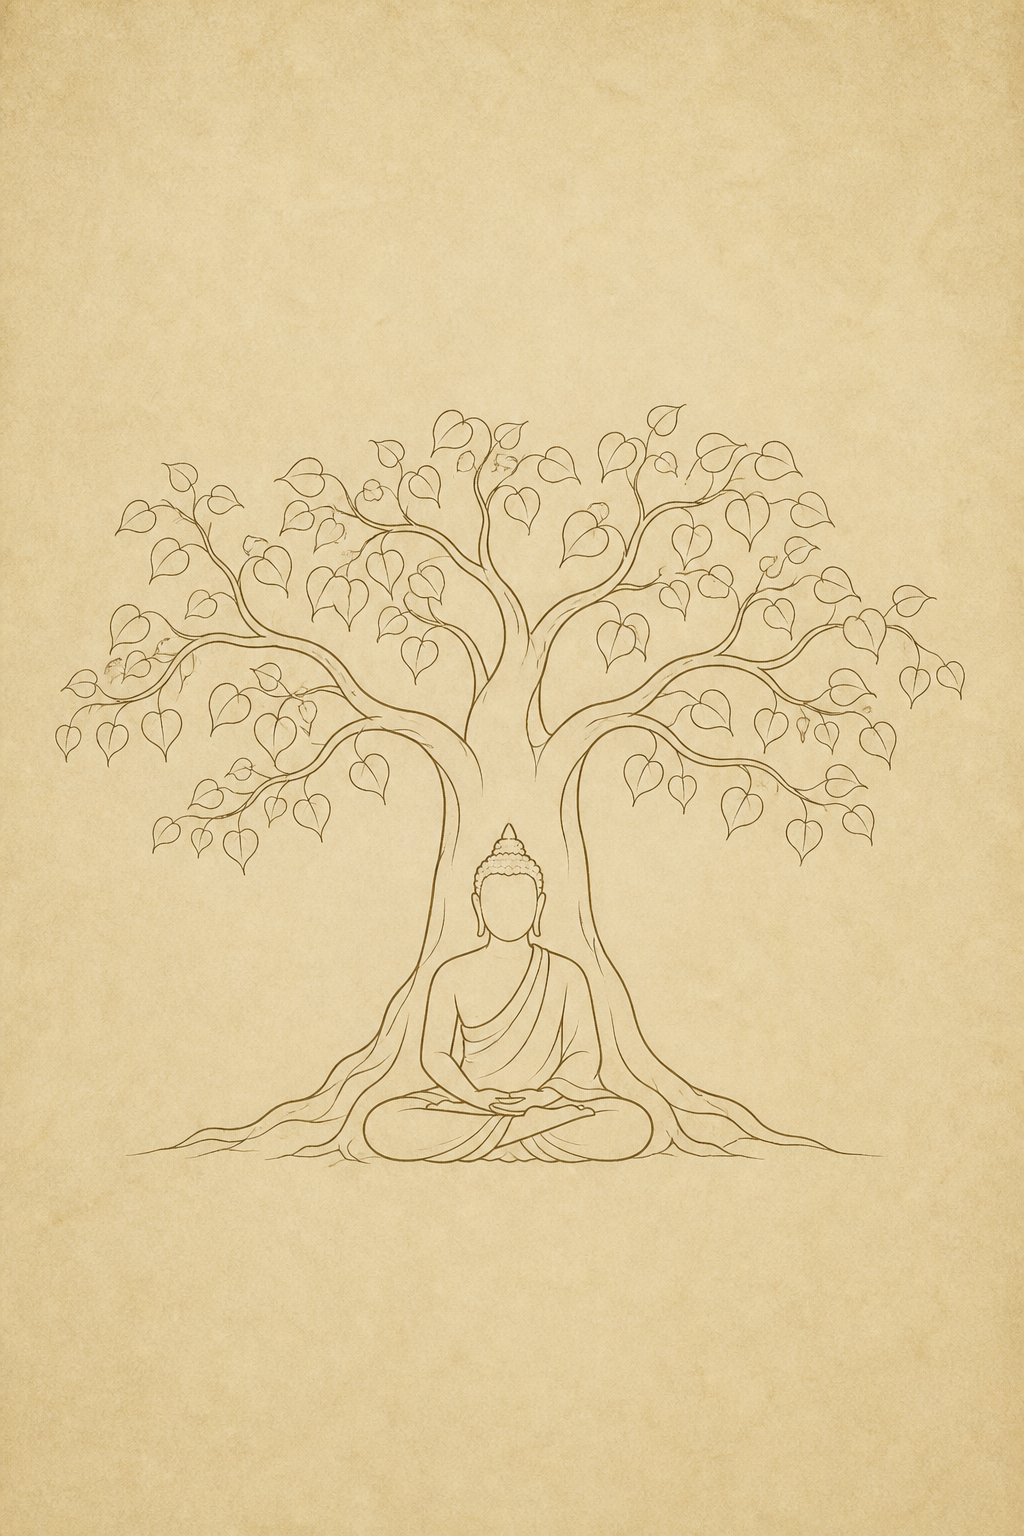
\includegraphics[width=0.58\textwidth]{../book/assets/cover.png}
\vfill
{\large\color{coverink} Saṃyukta Āgama\par}
\vspace{0.25em}
{\normalsize\color{coverink} A Kumarajiva-Style Research Translation\par}
\vspace{0.35em}
{\normalsize\color{coverink} Fascicle Order Reconstructed\par}
\vspace{0.8em}
{\normalsize\color{coverink} Agama–Kumarajiva Project · 2026\par}
\vspace{1.2cm}
\end{titlepage}
\nopagecolor
